%%%%%%%%%%%%%%%%%%%%%%%%%%%%%%%%%%%%%%%%%%%%%%%%%%%%%%%%%%%%%%%%%%%%%%%%%%%%%%%
\chapter{Experimental setup and results}~\label{chap:results}
%%%%%%%%%%%%%%%%%%%%%%%%%%%%%%%%%%%%%%%%%%%%%%%%%%%%%%%%%%%%%%%%%%%%%%%%%%%%%%%

A Linux kernel module as shown in Figure~\ref{fig:entire_seeker} was developed incorporating the ideas 
discussed in chapters \ref{chap:pds} and \ref{chap:delta}. 
The scheduling routines in the Linux kernel (To be specific, \textit{schedule} and \textit{\_\_switch\_to})
were extended using kprobes \cite{kprobes} to add the performance directed scheduling features.
The choice to use kprobes \cite{kprobes} a feature essentially used for debugging and instrumentation
from the context of a kernel module pose two possible 
problems. One, kprobes by themselves introduce unnecessary code paths and interrupts causing some
if not significant overhead (Less than 3\%). Secondly, certain functions relating to migration are not exported
to kernel modules and hence indirect and suboptimal procedures were chosen to get the necessary 
functionality. In spite of these disadvantages, having the project as a kernel module accelerated 
the development process. 

For a system with \textit{M} total performance states and \textit{N} total processors, $\Delta$ can 
at most take a value of $N \times (M-1)$. Experiments were carried on a quad-core AMD Opteron (Barcelona),
and a patched version of the Linux 2.6.28 kernel. The logging interface as shown in Figure~\ref{fig:entire_seeker},
collects task specific and system wide statistics which enable in studying the behavior of both the performance
directed scheduler and the delta constrained mutator. The statistics collected by the logging system aided in 
the computation of total energy consumption of each processor for each run workload. In order to measure 
percentage slowdown, the six workloads mentioned in Appendix~\ref{app:benchmark}, were run with full clock speed
and recording their cumulative execution time. In order to estimate power and energy consumption, the power 
values mentioned in \cite{AMDPow} (Provided in Appendix~\ref{app:opteron} for convenience) were utilized 
to compute the average power and energy consumption. Appendix~\ref{app:mutation_timeline} displays the 
adaptation time line graph showcasing each of the two schedulers along with the delta constrained mutator.

The system call interface allows an application runtime (or an application) to provide hints to the scheduler
on the performance state demanded and allows compiler and runtime power optimizing frameworks to interact with the underlying
kernel based power optimizer to create a more robust system. The system call interface is beyond the scope 
of this text and will not be further discussed, but shown only as an example of possible extensions to the 
discussed power management system.

\begin{figure}[h!]
  \begin{center}
    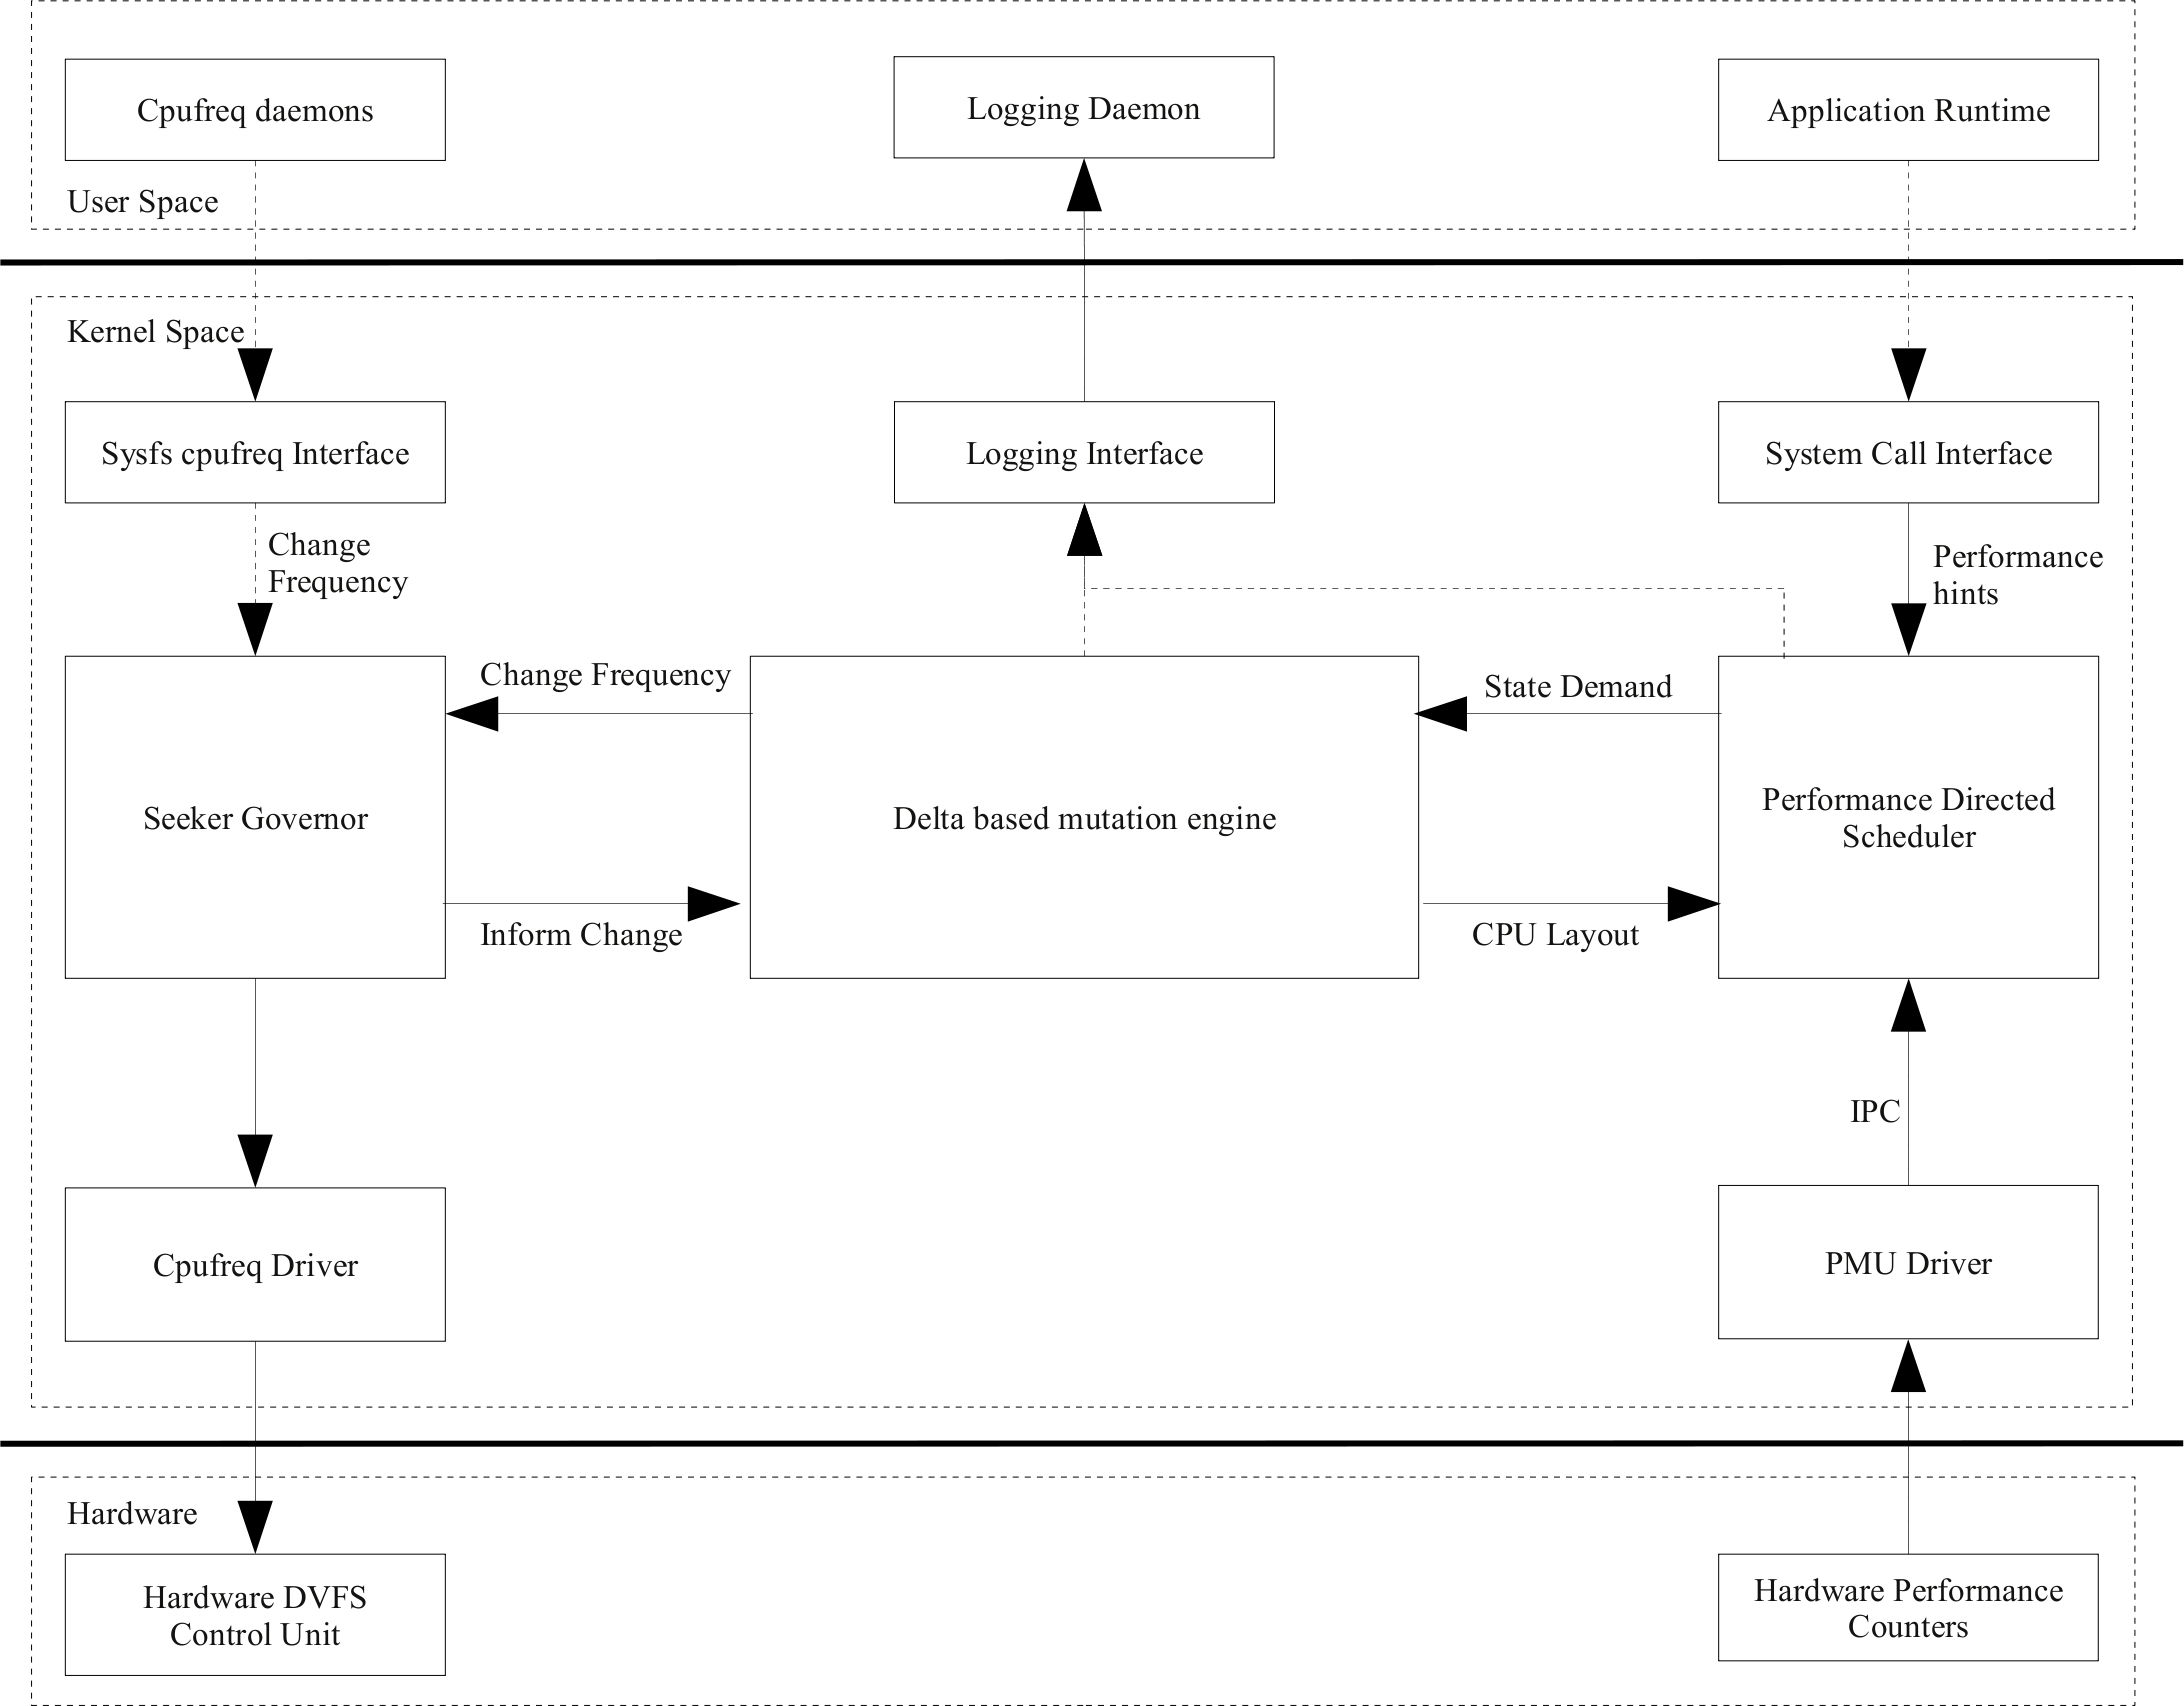
\includegraphics[height=4in]{figures/seeker.jpg}
    \caption{The Seeker infrastructure}
    \label{fig:entire_seeker}
  \end{center}
\end{figure}

%%%%%%%%%%%%%%%%%%%%%%%%%%%%%%%%%%%%%%%%%%%%%%%%%%%%%%%%%%%%%%%%%%%%%%
% START REAL GRAPHS
%%%%%%%%%%%%%%%%%%%%%%%%%%%%%%%%%%%%%%%%%%%%%%%%%%%%%%%%%%%%%%%%%%%%%%
%%%%%%%%%%%%%%%%%%%%%%%%%%%%%%%%%%%%%%%%%%%%%%%%%%%%%%%%%%%%%%%%%%%%%%%%%%%%%%%
\section{Trends along delta and interval}~\label{sec:trends}
%%%%%%%%%%%%%%%%%%%%%%%%%%%%%%%%%%%%%%%%%%%%%%%%%%%%%%%%%%%%%%%%%%%%%%%%%%%%%%%

Two parameters namely the delta constraint ($\Delta$) and the mutation interval 
were introduced in Chapter~\ref{chap:delta}. In order to further study the system
it is important to define the variation of two important effects,
namely, slowdown and power savings as a function of these parameters. In order
to accomplish the study, a fully factorial experiment was conducted varying delta 
from 1 through 16 and the interval from 125ms through 1000ms. All the six workloads in 
Table~\ref{tab:spec_groups} in Appendix~\ref{app:benchmark} were run in each 
experiment. Slowdown for each experiment was computed by comparing the execution time of each workload 
to that when run on a multi-processor system with all processors executing with the maximum frequency.


Figure~\ref{fig:slowdown_trends} show the trends
observed with respect to slowdown for the ladder and select schedulers. An unnaturally 
high slowdown can be observed for small values of delta ($\Delta$) and can be attributed
to the plasticity in adaptation. The interval of mutation has little significance towards slowdown
for delta values higher than 3 but when lowered beyond 3, the mutation interval begins to play a vital 
role in differentiating the experiments based on slowdown. It can be observed that at lower values
of delta, reducing the mutation interval has an effect of decreasing the slowdown and effectively 
reducing the performance lost. Comparing Figure~\ref{fig:slowdown_trends_ladder} 
with \ref{fig:slowdown_trends_select} shows that lower values of delta have a more profound negative 
effect on the select scheduling system than the ladder scheduling system. At $\Delta = 1$, the select scheduling
system exhibits at least 5\% increased in slowdown when compared to the ladder scheduling system but 
both rapidly falls to the plateau close to 16\% beyond a delta constraint of 4. 

\begin{figure}[h!]
\centering
  \subfigure[Ladder scheduler]{
    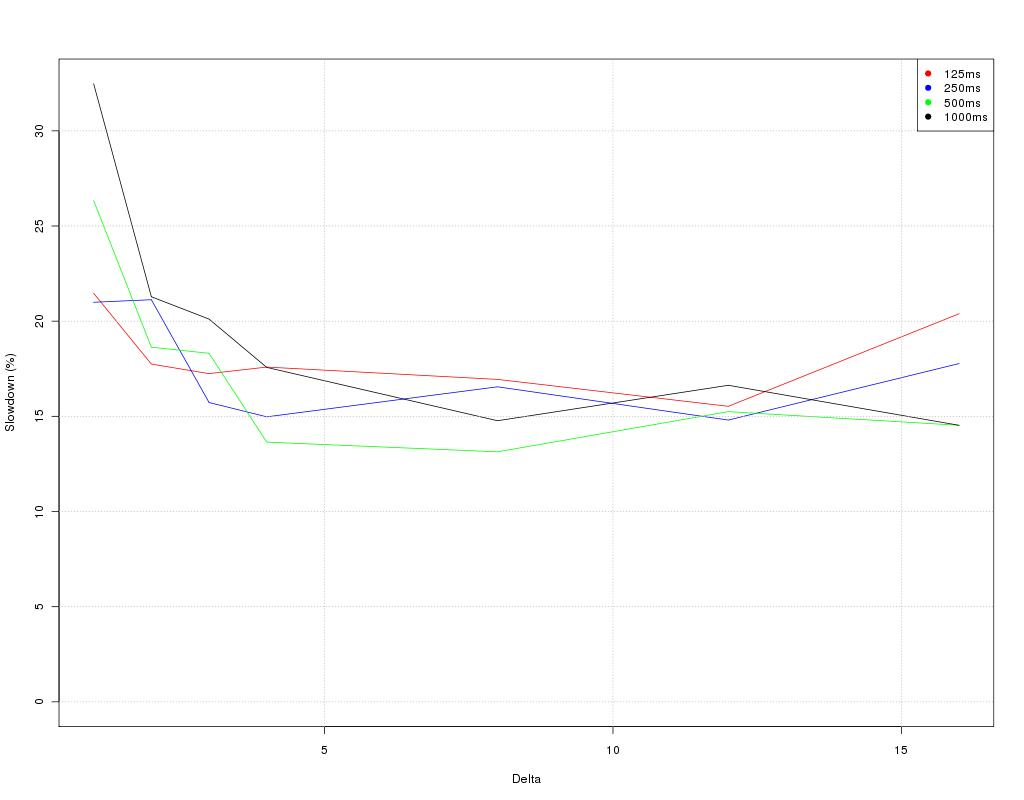
\includegraphics[height=2.5in]{figures/trends_slowdown_ladder.jpg}
    \label{fig:slowdown_trends_ladder}
  }
   \subfigure[Select scheduler]{
    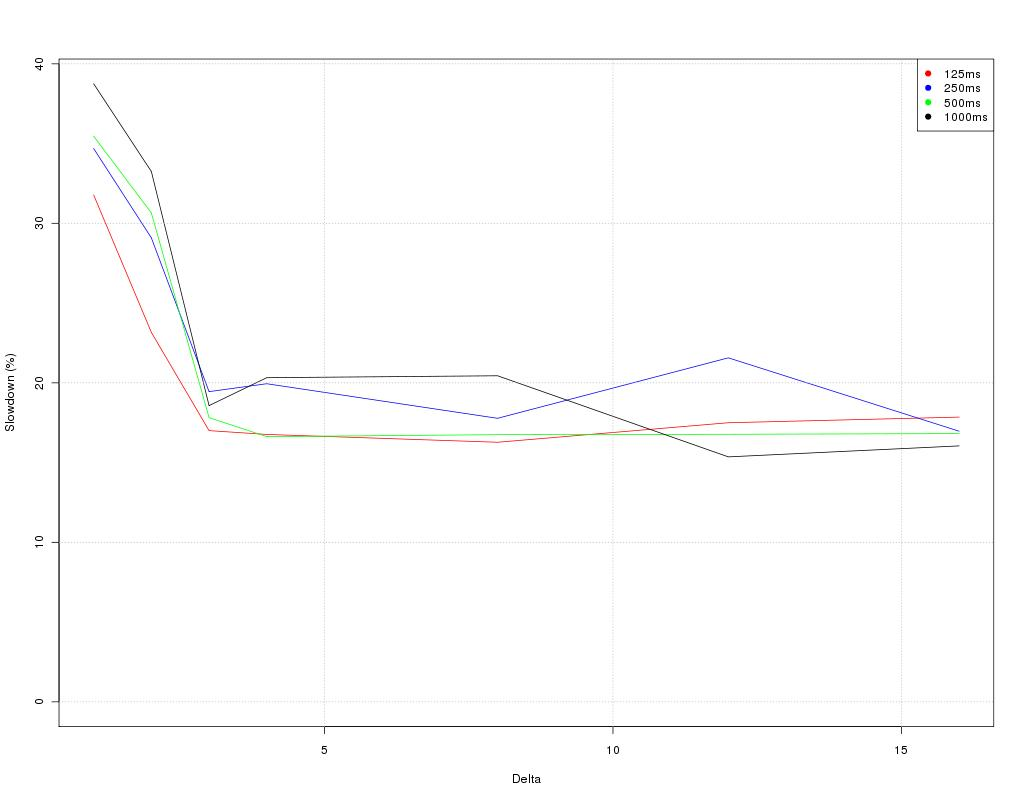
\includegraphics[height=2.5in]{figures/trends_slowdown_select.jpg}
    \label{fig:slowdown_trends_select}
  }
  \label{fig:slowdown_trends}
  \caption{Variation of slowdown with delta and interval for the ladder \subref{fig:slowdown_trends_ladder} and the select \subref{fig:slowdown_trends_select} scheduler}
\end{figure}

In order to study the power conservation, the logging interface was sampled to acquire
an execution sample's execution time and performance state (and in effect the power consumption
when compared to Table~\ref{tab:perf_power}). This allowed the measurement of the total 
energy consumption and along the execution time of each workload, the average power 
consumption was computed ($\text{Average power consumption} = \frac{\text{Total energy consumption}}{\text{total execution time}}$).
The percentage power savings is computed
by comparing the average power to the maximum power consumption (at the highest
frequency of 115.0W as shown in Table~\ref{tab:perf_power}).

Figure~\ref{fig:pwr_trends} shows the variation of percentage power savings with varied value 
of delta ($\Delta$) and mutation interval. A trend similar to percentage slowdown is observed
for power savings: A high value of power savings for lower values of delta which drop sharply 
at the value of $\Delta = 3$. Even though high power savings are desirable, the effective 
slowdown accompanying the delta constraint can be disadvantageous. A trend unique to power savings is the 
continued effect of mutation interval, whose decrease improves power savings marginally for all values of delta.
During the experimentation, mutation intervals lower than 100ms was observed to cause system
instabilities and frequent crashes and hence the study was performed only for values starting
from 125ms. Even though this phenomenon can be attributed to the implementation, \cite{ImpactDVFS} warns 
system designers to avoid rapid DVFS transitions and should not be ignored.


\begin{figure}[h!]
\centering
  \subfigure[Ladder scheduler]{
    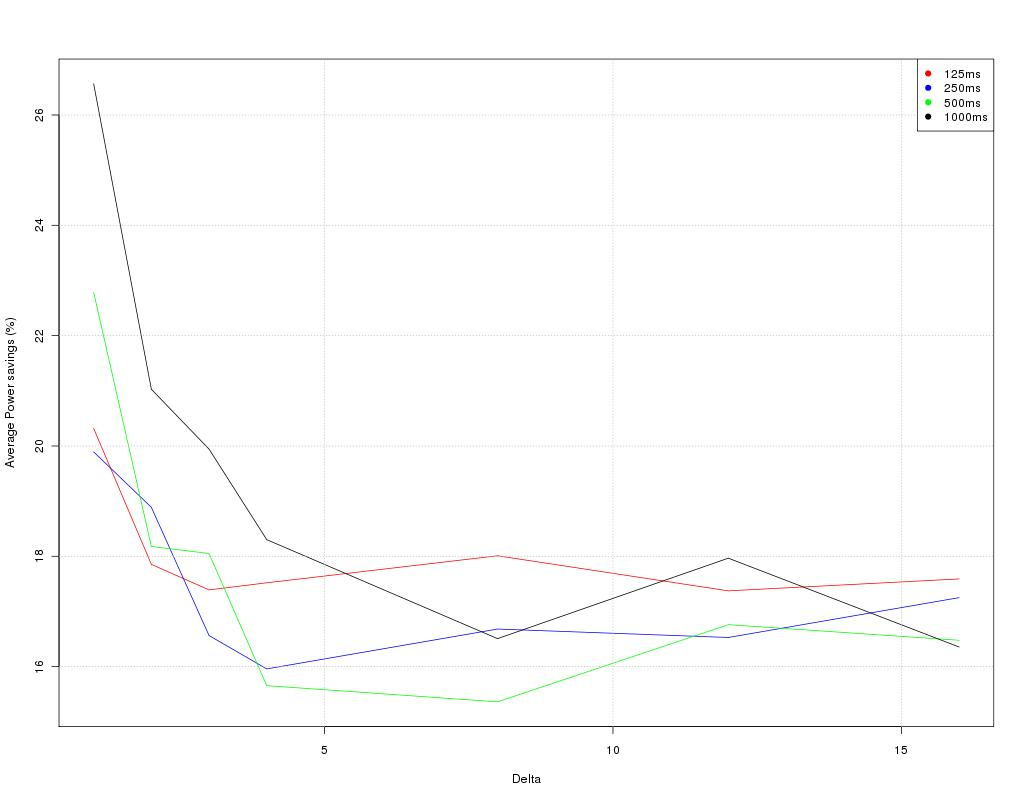
\includegraphics[height=2.5in]{figures/trends_avgpwr_ladder.jpg}
    \label{fig:pwr_trends_ladder}
  }
   \subfigure[Select scheduler]{
    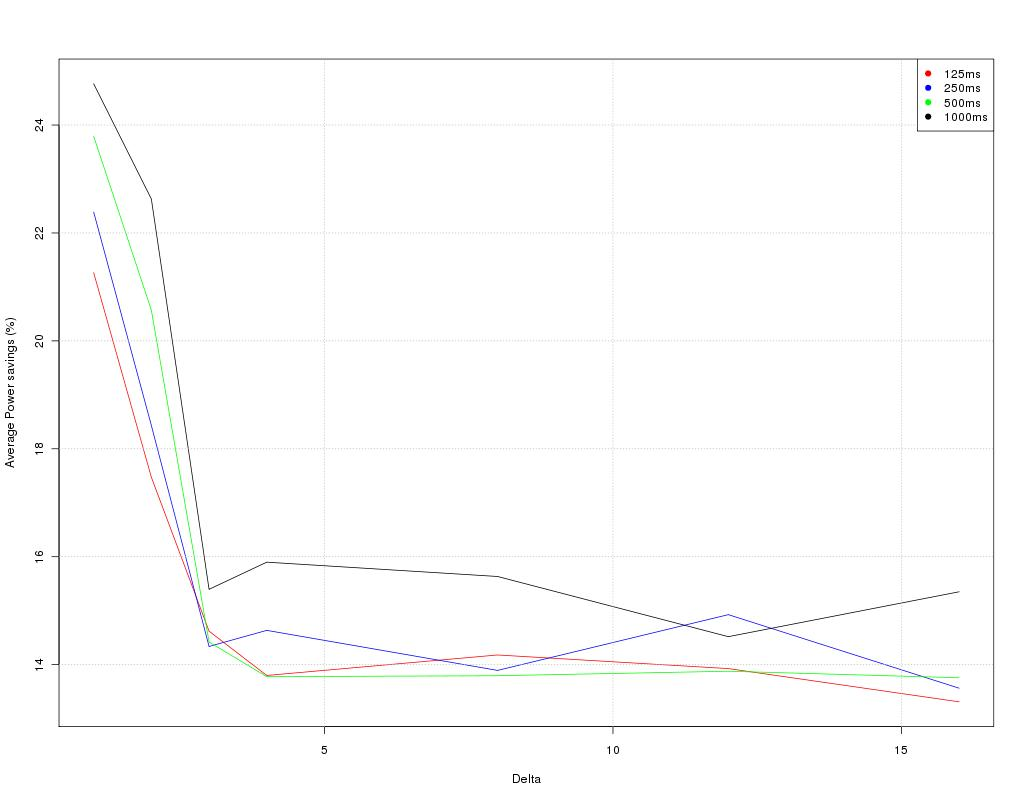
\includegraphics[height=2.5in]{figures/trends_avgpwr_select.jpg}%}
    \label{fig:pwr_trends_select}
  }
    \label{fig:pwr_trends}
    \caption{Variation of average power savings with delta and interval for the ladder (Subfigure~\subref{fig:pwr_trends_ladder}) and the select (Subfigure~\subref{fig:pwr_trends_select}) scheduler}
\end{figure}

Based on these observations, it can be concluded that a value of delta $\Delta = 4$ provides
the best among all the compromises and the interval can be changed based on the arrival rate
of jobs on the server or compute node. Having a very low mutation interval can hamper 
potential power savings for systems with a high mean time between execution workloads 
hence advising system designers to consider all parameters before deploying the delta
constrained mutator.

%%%%%%%%%%%%%%%%%%%%%%%%%%%%%%%%%%%%%%%%%%%%%%%%%%%%%%%%%%%%%%%%%%%%%%%%%%%%%%%
\section{Effects of workload on power and performance}~\label{sec:wrk_trends}
%%%%%%%%%%%%%%%%%%%%%%%%%%%%%%%%%%%%%%%%%%%%%%%%%%%%%%%%%%%%%%%%%%%%%%%%%%%%%%%

Due to the adaptive nature of the power management mechanism and the high dependence
on the IPC characteristic of workloads, it can be hypothesized
that workloads with lower IPC (The \textit{Low} workload) should expect the maximum
power savings while, workloads with large IPC (The \textit{High} workload) should
expect the minimum slowdown and power savings.
The slowdown and power savings box plots were drawing showcasing their characteristics and 
variation for each workload. It must be noted that the data from the experiments 
performed for the study presented in Section~\ref{sec:trends} were reused for the 
current analysis and was not pruned to the best values of delta and mutation interval. 
This enables the study of maximum impact of variation of these parameters
(delta and mutation interval) for each workload. 

Figure~\ref{fig:workload_trends} shows the variation of percentage slowdown and power savings 
for each workload with both the scheduler systems. The \textit{High} workload 
suffers the minimum performance loss at a median close to 0\%. This is due to the fact 
that the adaptive scheduling system adapts to its high IPC characteristic and rapidly
provides it processors with the highest possible clock speed and hence explaining 
the insignificant slowdown. On the other hand, the \textit{Low} workload suffers a slowdown
of close to 17\% while providing an excess of 40\% power savings for the ladder scheduling
system. As the characteristic of the \textit{Low} workload is an average value of IPC below 0.5, 
the ladder system rapidly adapts to providing the workload the lowest clock speed and 
in turn conserving power. This displays the advantage of a workload based power optimizing 
system where the clock speed can be reduced by half its value and still certain workloads
can suffer at the most 20\% slowdown but providing up to 50\% in power savings. 

As the select scheduling system provides the \textit{Low} workload a higher clock speed than the 
ladder scheduling system (Observable in Appendix~\ref{app:mutation_timeline}, 
Figures~\ref{fig:wrk_low_ladder} and \ref{fig:wrk_low_select}), the power savings is 
noticeable lower. A high variance of slowdown can be observed for the \textit{High} 
workload running on the select scheduler indicating the cause of the additional slowdown
suffered by the select scheduling system when compared to the ladder system.

\begin{figure}[h!]
\centering
  \subfigure[Ladder scheduler]{
    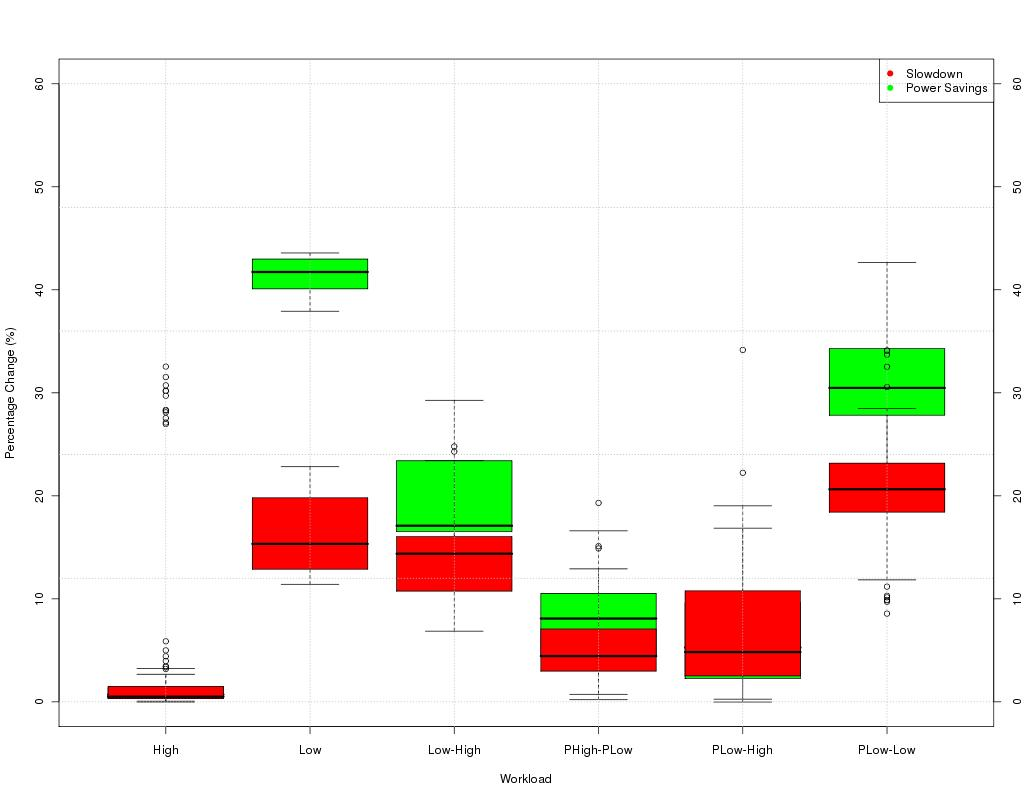
\includegraphics[height=2.5in]{figures/trends_workload_ladder.jpg}%}
    \label{fig:workload_trends_ladder}
  }
   \subfigure[Select scheduler]{
    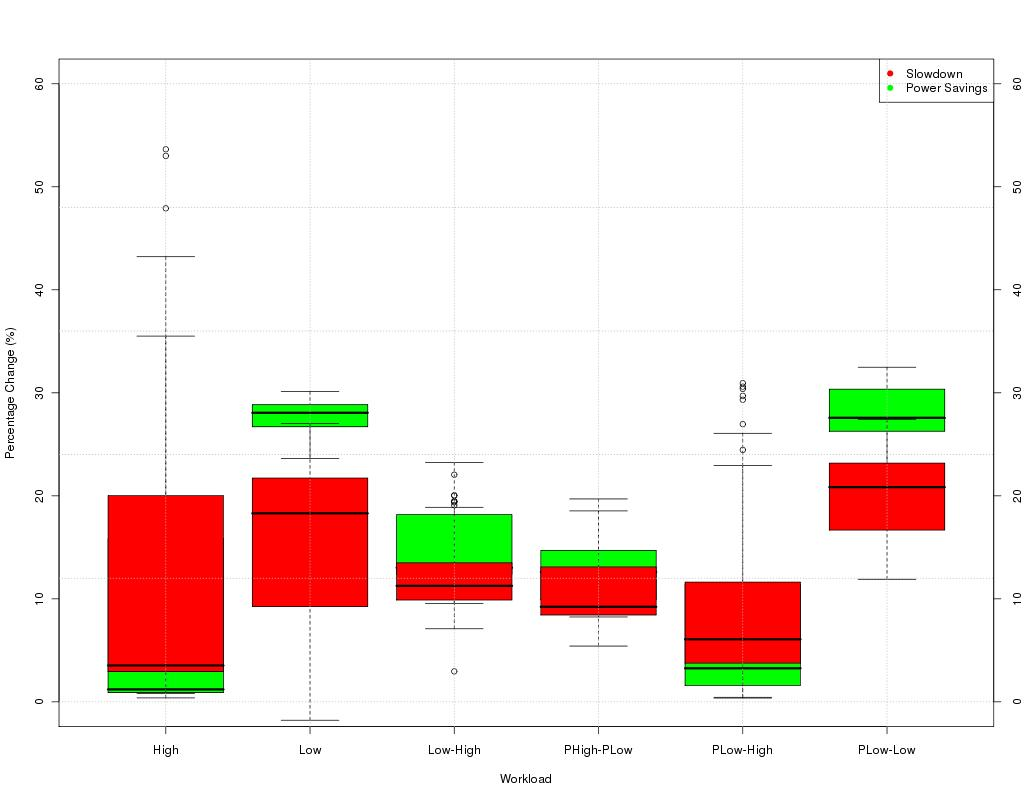
\includegraphics[height=2.5in]{figures/trends_workload_select.jpg}%}
    \label{fig:workload_trends_select}
  }
\label{fig:workload_trends}
\caption{Variation of slowdown and power savings for each workload for the ladder (Subfigure~\subref{fig:workload_trends_ladder}) and the select (Subfigure~\subref{fig:workload_trends_select}) scheduler}
\end{figure}

%%%%%%%%%%%%%%%%%%%%%%%%%%%%%%%%%%%%%%%%%%%%%%%%%%%%%%%%%%%%%%%%%%%%%%%%%%%%%%%
\section{Comparing various methodologies}~\label{sec:compare}
%%%%%%%%%%%%%%%%%%%%%%%%%%%%%%%%%%%%%%%%%%%%%%%%%%%%%%%%%%%%%%%%%%%%%%%%%%%%%%%

Chapter~\ref{chap:pds} described two methods of evaluating the performance state and hence
providing two distinct methods of scheduling affecting the adaptation of the delta system.
Chapter~\ref{chap:delta} introduced a common power management system, the \textit{ondemand}
power optimizer. Experiments were conducted varying the mutation interval from 125ms to
1000ms for all three systems. Section~\ref{sec:trends} recommends the minimum value of 
delta $\Delta = 4$ in order to minimize the effects of slowdown due to adaptation plasticity
and hence the delta mutator with a value of $\Delta = 4$ was utilized for the experiments
proposed in this section. 
Utilizing the logging interface, the execution sample 
performance state (and in turn the power consumption), execution time and retired instructions 
were recorded to later compute the average power consumption for each workload, the energy
efficiency, measured as energy consumption per executed instruction and slowdown. 
These experiments were repeated for each of the power management systems:
\begin{itemize}
\item Ondemand governor, mutation interval: 125ms, 250ms, 500ms, 1000ms
\item The ladder performance directed scheduling system with the delta constrained mutator with 
a delta value, $\Delta = 4$ and mutation interval: 125ms, 250ms, 500ms, 1000ms
\item The select performance directed scheduling system with the delta constrained mutator with 
a delta value, $\Delta = 4$ and mutation interval: 125ms, 250ms, 500ms, 1000ms
\end{itemize}
For each experiment, the percentage power savings, percentage slowdown and EPI (energy per instruction)
was computed and tabulated. These experiments were clustered based on workload in order to further 
categorize the results.

Figure~\ref{fig:pwr_vs_slowdown} shows a scatter plot of slowdown plotted against power savings. Each point
represents an experiment/workload and differentiated based on workload. 
Points lower indicate smaller magnitude of slowdown while points farther to the right indicate better power
savings. This graph clearly shows the vice of the Ondemand governor: It does not manage power at active
load (obvious from it's design considerations). This is graphically depicted by all the points pertaining
to the ondemand governor huddled around Power Savings = 0\% and hence providing absolutely no power savings
while the processors are actively executing jobs. The Delta + Select system provides an equal power savings
as the Delta + Ladder except for the workload \textit{Low} for which the ladder system works better in achieving
higher power savings for equal values of slowdown.

\begin{figure}[h!]
  \begin{center}
    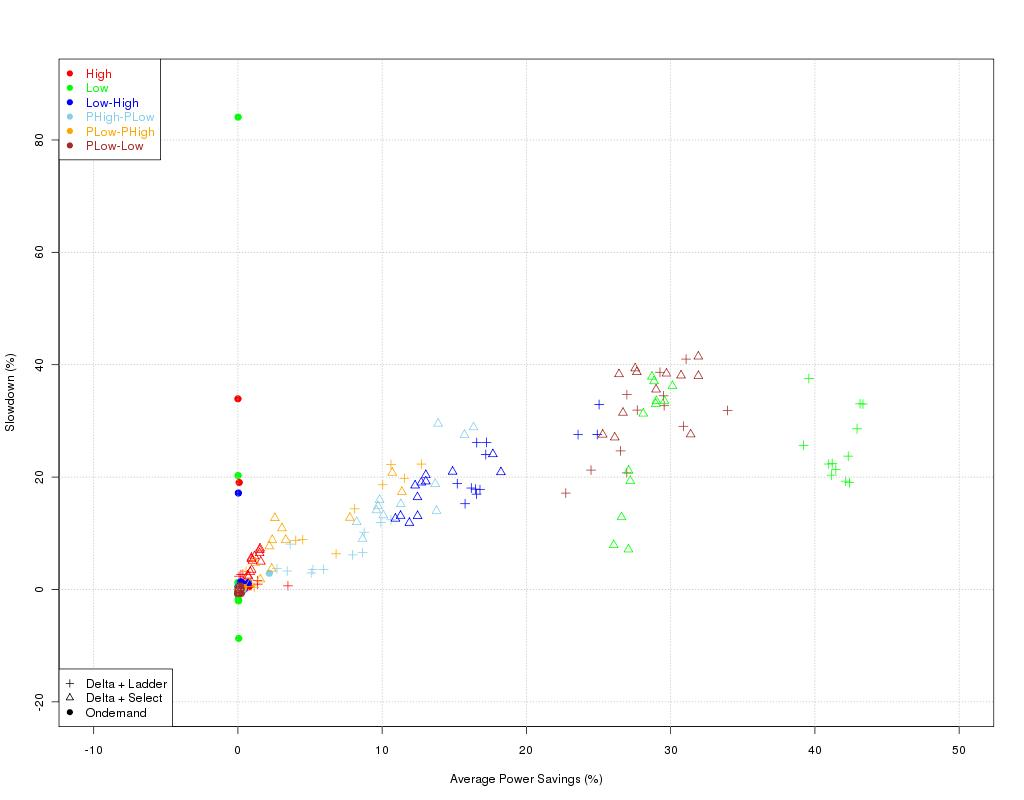
\includegraphics[height=3.0in]{figures/pwr_vs_slowdown_delta_4.jpg}
    \caption{Scatter plots showing variation of slowdown with power savings for ondemand, $\Delta=4$ (Select and Ladder)}
    \label{fig:pwr_vs_slowdown}
  \end{center}
\end{figure}

EPI (Energy consumption per instruction) is another important metric which ties in bother throughput and power
consumption with lower values indicating better energy efficiency. EPI is plotted 
against power savings for each experiment to arrive at Figure~\ref{fig:pwr_vs_jpbi}. As the ondemand governor
does not manage power at execution time, it is observed that not only does it not provide any power savings, 
it ends up utilizing energy inefficiently. Note that the value of EPI for the ondemand governor can be as high
as 170 nW/instruction while both the ladder and select systems exhibit a max EPI of 140 nW/instruction. 
Figure~\ref{fig:pwr_vs_jpbi} also displays the linear relationship between EPI and power savings introduced
by both the select and ladder systems.

\begin{figure}[h!]
  \begin{center}
    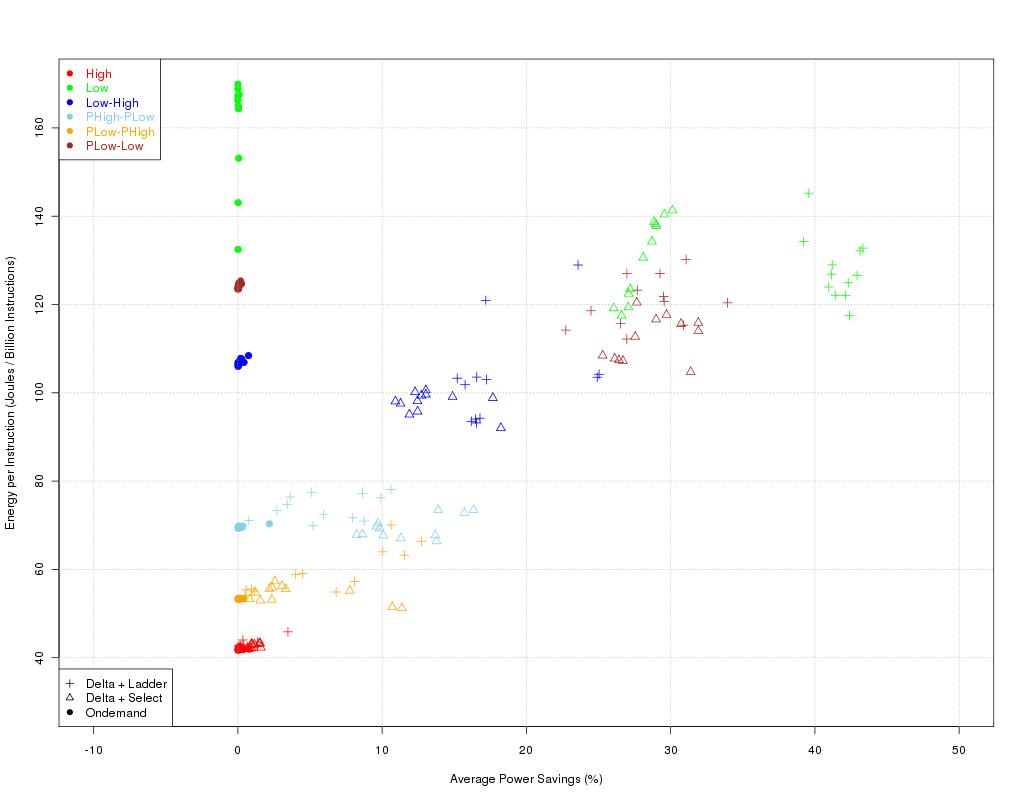
\includegraphics[height=3.0in]{figures/pwr_vs_jpbi_delta_4.jpg}
    \caption{Scatter plots showing variation of EPI with power savings for ondemand, $\Delta=4$ (Select and Ladder)}
    \label{fig:pwr_vs_jpbi}
  \end{center}
\end{figure}


An interesting graph Figure~\ref{fig:jpbi_vs_slowdown} is arrived at when the scatter plots concentrate on
EPI and slowdown. As we have concluded with figures \ref{fig:pwr_vs_slowdown} and \ref{fig:pwr_vs_jpbi},
the ondemand governor essentially executes all workloads at the highest clock speed (Indicated by 0\% slowdown 
and power savings). This allows \ref{fig:jpbi_vs_slowdown} to be viewed to discern if the delta system
does provide a better means to execute workloads in a more energy efficient manner. This is observable
where all the points for each workload pertaining to the delta + select and delta + ladder systems lie to the left of their
respective points for the points pertaining to the ondemand power optimizer. A conclusion based on 
Figure~\ref{fig:jpbi_vs_slowdown} can be made to assert the fact that the delta mutation system is more 
energy efficient than the ondemand system and equal at worst.

\begin{figure}[h!]
  \begin{center}
    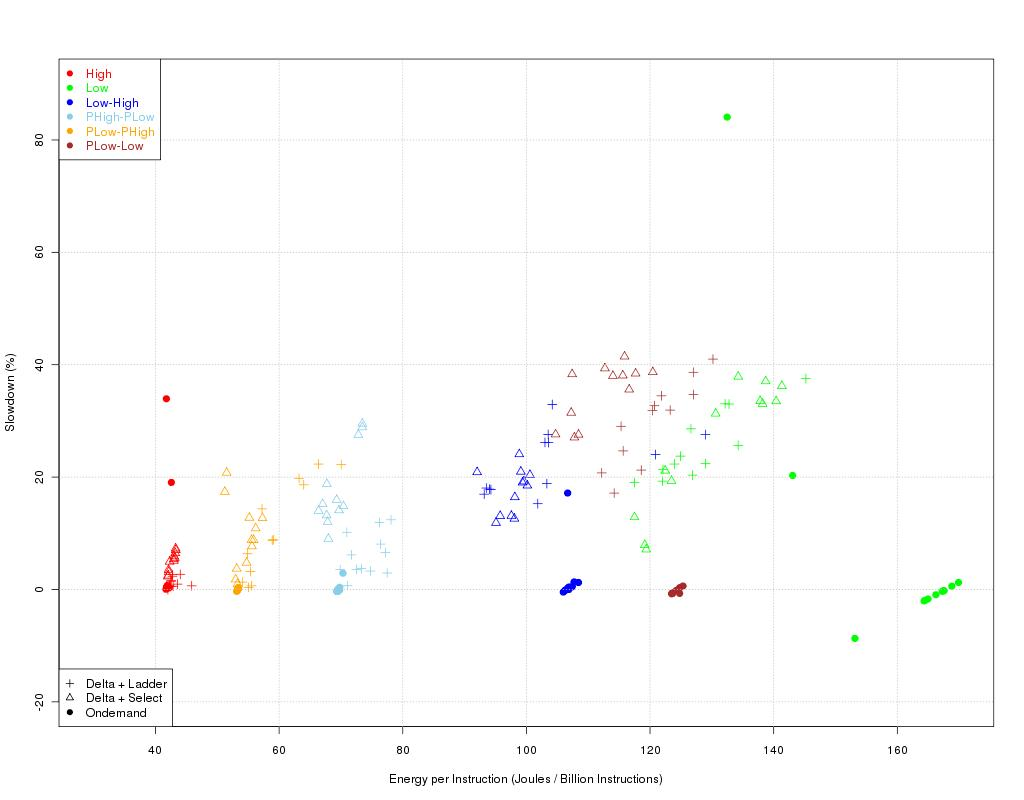
\includegraphics[height=3.0in]{figures/jpbi_vs_slowdown_delta_4.jpg}
    \caption{Scatter plots showing variation of slowdown with EPI for ondemand, $\Delta=4$ (Select and Ladder)}
    \label{fig:jpbi_vs_slowdown}
  \end{center}
\end{figure}

%%%%%%%%%%%%%%%%%%%%%%%%%%%%%%%%%%%%%%%%%%%%%%%%%%%%%%%%%%%%%%%%%%%%%%%%%%%%%%%
\section{Power savings and slowdown}~\label{sec:pow_slow}
%%%%%%%%%%%%%%%%%%%%%%%%%%%%%%%%%%%%%%%%%%%%%%%%%%%%%%%%%%%%%%%%%%%%%%%%%%%%%%%

The power optimizing system described in Chapters~\ref{chap:pds} and \ref{chap:delta} are shown
to introduce slowdown and hence deteriorate performance. This section describes experiments 
performed to estimate the relationship between slowdown and power savings. Each of the six
workloads were executed on both the ladder and the select systems with varying parameters
(delta from 3 to 16, and mutation interval from 125ms to 1000ms). The results of the experiments
were plotted with power savings as a function of slowdown in order to characterize potential 
power savings for arbitrarily observed slowdown. The data was estimated as a linear function
using a linear regression model shown in Figure~\ref{fig:regression}. The scatter plots along
with the regression model for the ladder and select scheduling system is shown in Figures~\ref{fig:slowdown_power_ladder}
and \ref{fig:slowdown_power_select} displaying the accuracy of the regression model. 

\begin{figure}[h!]
   \begin{equation*}
      \text{Power Savings (Ladder)} = (1.003 \times \text{Slowdown}) + 0.935
    \end{equation*}
    \begin{equation*}
     \text{Power Savings (Select)}  = (0.783 \times \text{Slowdown}) + 0.416
  \end{equation*}
  \caption{Regression models for the ladder and select scheduling systems}
  \label{fig:regression}
\end{figure}

\begin{figure}[h!]
  \begin{center}
    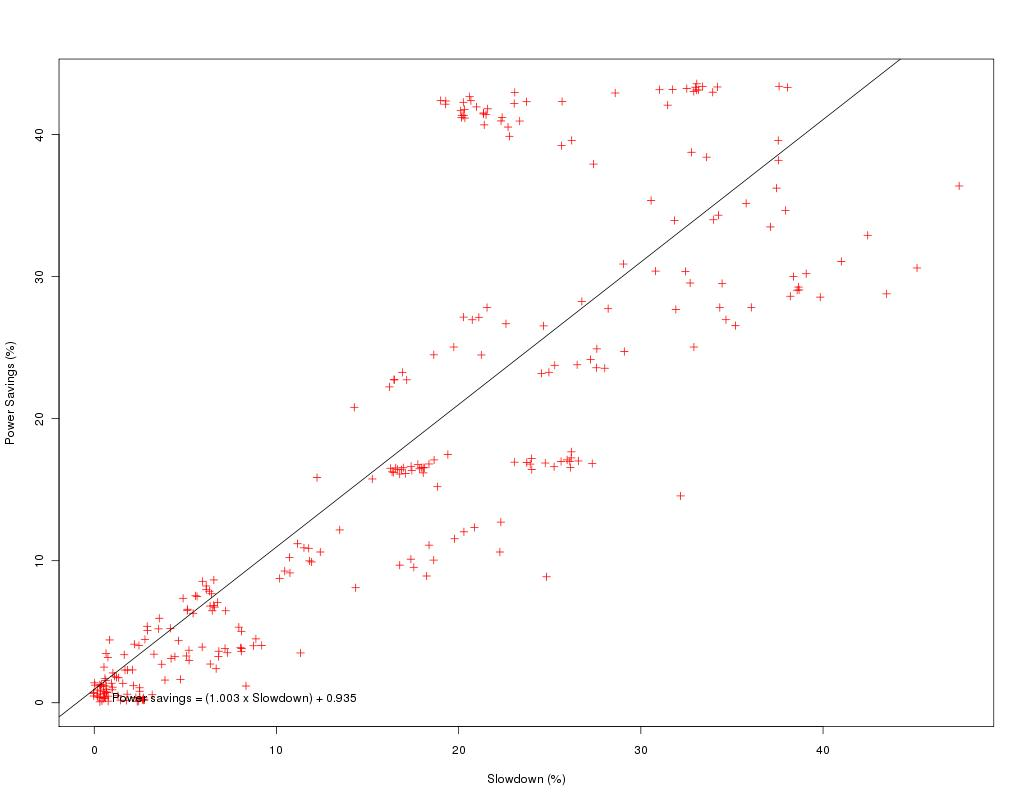
\includegraphics[height=3.0in]{figures/slowdown_power_ladder.jpg}
    \caption{Trends over workload variation}
    \label{fig:slowdown_power_ladder}
  \end{center}
\end{figure}

\begin{figure}[h!]
  \begin{center}
    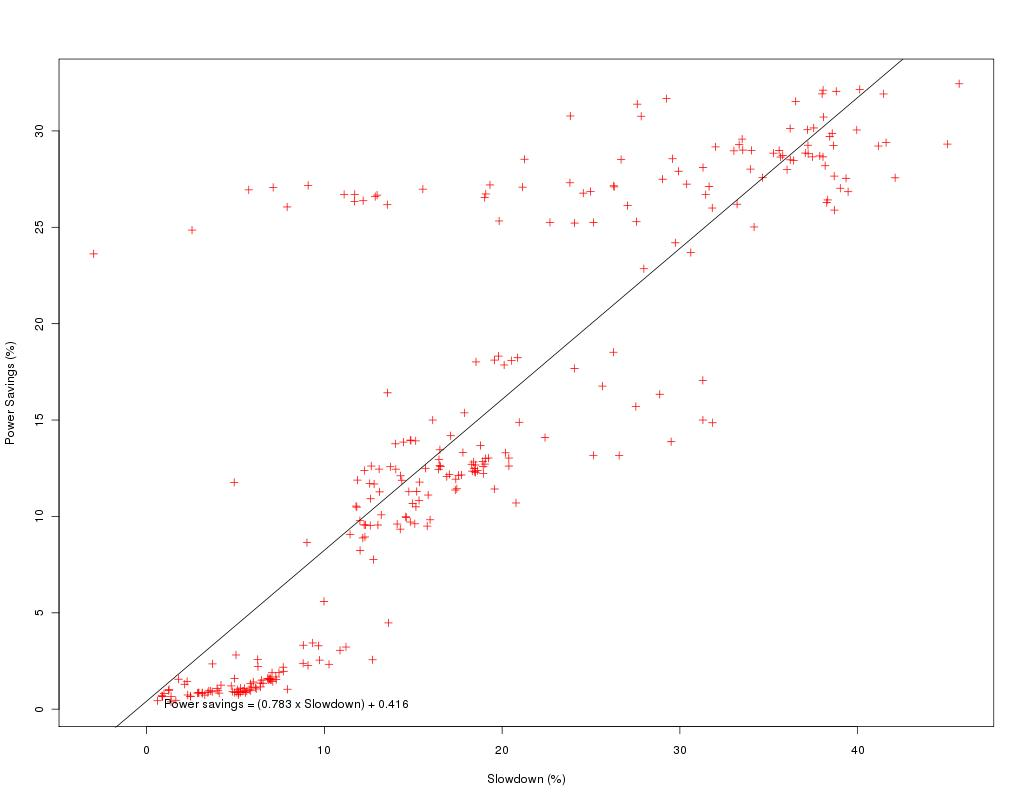
\includegraphics[height=3.0in]{figures/slowdown_power_select.jpg}
    \caption{Trends over workload variation}
    \label{fig:slowdown_power_select}
  \end{center}
\end{figure}

It can be observed that the ladder scheduling system along with the delta constrained mutator 
provide equal amount of power savings for every percentage of performance lost while a lower 
value of around 0.8\% of power savings can be expected from the select scheduling system for
the same amount of performance lost. Note that these are descriptive models to provide a
workload agnostic view of the power management system and are not real behavior as larger
power savings were achieved with minimum performance loss as demonstrated in earlier sections. 